\documentclass[12pt,aspectratio=169]{beamer}

\mode<presentation>
{
  \usetheme{Singapore}
 %\setbeamersize{text margin left=.6cm,text margin right=.6cm}
%  \setbeamertemplate{navigation symbols}{} % suppress nav bar
%  \setbeamercovered{transparent}
}
\usefonttheme{professionalfonts}
\usepackage{graphicx}
\usepackage{tikz}
\usepackage{amsmath}
\usepackage{mathpazo}
\usepackage[scaled]{helvet}
\usepackage{xcolor,colortbl}
\usepackage{siunitx}
\usepackage[siunitx]{circuitikz} % to draw circuits!

\sisetup{number-math-rm=\mathnormal}

\title{Classes 14 \& 15: Magnetism, Part 2}
\subtitle{AP Physics}
\author[TML]{Dr.\ Timothy Leung}
\institute{Olympiads School}
\date{February 2018}

\newcommand{\pic}[2]{\includegraphics[width=#1\textwidth]{#2}}
\newcommand{\mb}[1]{\mathbf{#1}}
\newcommand{\eq}[2]{\vspace{#1}{\Large\begin{displaymath}#2\end{displaymath}}}
\newcommand{\protip}[1]{
  \begin{center}
    \fbox{
      \begin{minipage}{.95\textwidth}
        {\footnotesize
          \textbf{Protip: }#1
        }
      \end{minipage}
    }
  \end{center}
}

\begin{document}

\begin{frame}
  \maketitle
\end{frame}


%\section[Intro]{Introduction}

\begin{frame}
  \frametitle{Files for You to Download}
  Download from the school website:
  \begin{enumerate}
  \item\texttt{14-Magnetism2.pdf}---The ``print version'' of this
    presentation. If you want to print the slides on paper, I recommend
    printing 4 slides per page.
%  \item\texttt{14-Homework.pdf}---Homework assignment for Class 14.
%    Please note the new formatting style
  \end{enumerate}

  \vspace{.2in}Please download/print the PDF file before each class. When you
  are taking notes, pay particular attention to things I say that aren't
  necessarily on the slides.
\end{frame}

\section{Magnetic Flux}


\begin{frame}
  \frametitle{Magnetic Flux}

  \textbf{Question:} If a current-carrying wire can generate a magnetic field,
  can a magnetic field affect the current in a wire?

  \vspace{.3in}\textbf{Answer:} Yes, sort of\ldots

  \vspace{.3in}To understand how to \emph{induce} a curent by a magnetic field,
  we need to look at fluxes again.
\end{frame}

\begin{frame}
  \frametitle{Magnetic Flux}
  \begin{columns}
    \column{.4\textwidth}
    \pic{1.1}{flux2.png}
  
    \column{.6\textwidth}
    Magnetic flux is defined as:
    
    \eq{-.15in}{
      \boxed{\Phi_\mathrm{magnetic}=\int\mb{B}\cdot d\mb{A}}
    }
    
    \vspace{-.1in}where $\mb{B}$ is the magnetic field, and $d\mb{A}$ is the
    infinitesimal area pointing \textbf{outwards}. If you are uncomfortable
    with using vector surfaces, note that magnetic flux can also be expressed
    as:

    \eq{-.15in}{
      \boxed{\Phi_\mathrm{magnetic}=\int\mb{B}\cdot\hat{\mb{n}}dA}
    }

    \vspace{-.1in}where $\hat{\mb{n}}$ is the outward normal direction
  \end{columns}
\end{frame}


\begin{frame}
  \frametitle{Magnetic Flux Over a Closed Surface}

  The unit for magnetic flux is a ``weber'' (\si{\weber}), in honor of
  German physicist Wilhelm Weber, who invented the electromagnetic
  telegraph with Carl Gauss. It is defined as:

  \eq{-.3in}{\SI{1}{\weber}=\SI{1}{\tesla.\metre^2}}
  
  \vspace{-.2in}The magnetic flux over a closed surface is always zero:

  \eq{-.2in}{
    \boxed{\oint\mb{B}\cdot d\mb{A}=0}
  }

  \vspace{-.1in}Since magnetic field lines only exist as a loop, that means
  there should be equal amount of ``flux'' flowing out of a closed surface as
  entering the surface.
\end{frame}


\section{Faraday's Law}
\begin{frame}
  \frametitle{Changing Flux}
  We can 

  Unlike in a basic circuit, where the \emph{emf} is concentrated at the
  terminals of the battery, the induced \emph{emf} is spread across the entire
  wire.

\end{frame}

\begin{frame}
  \frametitle{Faraday's Law}
  Faraday's law states that the rate of change of magnetic flux produces an
  electromotive force:

  \eq{-.3in}{
    \boxed{\mathcal{E}=\oint\mb{E}\cdot d\mb{l}=-\frac{d\Phi}{dt}}
  }
\end{frame}

\begin{frame}
  \frametitle{How Can Magnetic Flux Change}
  Magnetic flux can change due to a number of reasons:
  \begin{enumerate}
  \item\textbf{Changing magnetic field strength} e.g.\  if $\mb{B}$ is created
    by a time dependent current source like an alternating current
  \item\textbf{Changing orientation of magnetic field} because the
    surface area is moving (translation and/or rotation) relative to $\mb{B}$
  \item\textbf{Changing area} the surface area from which the flux is
    calculated is changing
  \end{enumerate}
\end{frame}



\section{Lenz's Law}



\section{Motional EMF}



\section{Generators and Motors}



\section{Inductance}

\begin{frame}
  \frametitle{Self Inductance}
  A solenoid carrying a current generates a magnetic field; its strength given
  by Biot-Savart Law.
  \begin{center}
    \textbf{MISSING DIAGRAM HERE!}
  \end{center}
  Since $\mb{B}\propto I$, the magnetic flux through the coil is therefore also
  proportional to $I$, i.e.:

  \eq{-.35in}{\boxed{\Phi_\text{magnetic}=LI}}

  \vspace{-.1in}where $L$ is the called the \textbf{self inductance} of the
  coil.
\end{frame}


\begin{frame}
  \frametitle{Self Inductance}

  For a solenoid, we can see that the self inductance is given by:

  \eq{-.2in}{
    \boxed{L=\frac{\Phi_{\textrm{magnetic}}}{I}=\mu_0 n^2Al}
  }

  where $\mu_o$ is the magnetic permeability of free space, $n$ is the number of
  coil turns per unit length, and $A$ and $l$ are the cross-section and length
  of the solenoid. (i.e. $Al$ is the enclosed volume.)
\end{frame}


\begin{frame}
  \frametitle{Self Inductance and Induced EMF}
  If the current changes, the magnetic flux changes as well, therefore inducing
  an electromotive force in the circuit! According Faraday's law:

  \eq{-.2in}{
    \boxed{\mathcal{E}=-\frac{d\Phi}{dt}=-L\frac{dI}{dt}}
  }

  The self-induced emf is proportional to the rate of change of current.
\end{frame}


\begin{frame}
  \frametitle{Mutual Inductance}

\end{frame}



\section{LR Circuits}

\begin{frame}
  \frametitle{Circuits with Inductors}
  \begin{itemize}
  \item Coils and solenoids in circuits are known as ``inductors'' and have
    large self inductance $L$
  \item Self inductance prevents currents rising and falling instantaneously
  \item A basic circuit containing a resistor and an inductor is called an
    \textbf{\emph{LR} circuit}:
    \begin{center}
      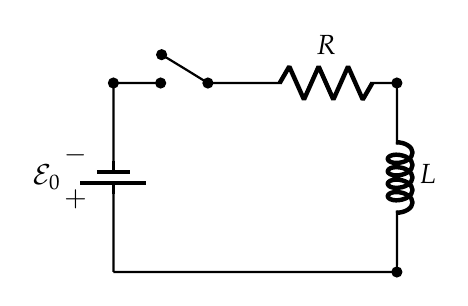
\begin{tikzpicture}[american voltages,scale=1.2]
        \draw[thick](0,0) to[battery1=$\mathcal{E}_0$,-*] (0,2)
        to[short,-*](0.5,2);
        \draw[thick](0.51,2.3) to[short,*-*](1,2)--(1.5,2) to [R=$R$,-*] (3,2)
        to [L=$L$,-*] (3,0)--(0,0);
      \end{tikzpicture}
    \end{center}
  \end{itemize}
\end{frame}

\begin{frame}
  \frametitle{Analyzing LR Circuits}
  \begin{columns}
    \column{.35\textwidth}
    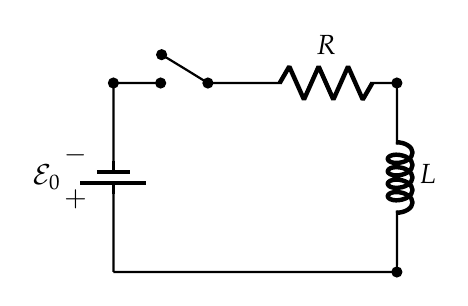
\begin{tikzpicture}[american voltages,scale=1.2]
      \draw[thick](0,0) to[battery1=$\mathcal{E}_0$,-*] (0,2)
      to[short,-*](0.5,2);
      \draw[thick](0.51,2.3) to[short,*-*](1,2)--(1.5,2) to [R=$R$,-*] (3,2)
      to [L=$L$,-*] (3,0)--(0,0);
    \end{tikzpicture}

    \column{.65\textwidth}
    Applying Kirchkoff's voltage law:

    \eq{-.2in}{\mathcal{E}_0-IR-L\frac{dI}{dt}=0}

    \vspace{-.1in}We follow the same procedure as charging a capacitor to find
    the time dependent current:

    \eq{-.2in}{I=\frac{\mathcal{E}_0}{R}\left(1-e^{-Rt/L}\right)}

    \vspace{-.15in} The time constant for an $LR$ circuit is
    
    \eq{-.2in}{\tau=\frac{L}{R}}
  \end{columns}
\end{frame}




\begin{frame}
  \frametitle{Magnetic Energy}
  Just as a capacitor stores energy, the energy stored by an inductor carrying
  a current $I$ in given by:

  \eq{-.2in}{ \boxed{U_m=\frac{1}{2}LI^2}}
  
\end{frame}




\section{Maxwell's Equations}
\begin{frame}
  \frametitle{Maxwell's Equations in Integral Form}
  James Clerk Maxwell recognized the relationship between electricity and
  magnetism, and combined the few laws into a unifying set of equations, now
  known as \textbf{Maxwell's equations} for electrodynamics:


  By manipulating the equations, we can show the existence of a
  ``electromagnetic wave'' that travels at the speed of light.
\end{frame}

\begin{frame}
  \frametitle{Maxwell's Equations in Differential Form}
\end{frame}

\end{document}
